\begin{frame}
  \frametitle{Задача <<День рождения>>}
  \begin{center}
    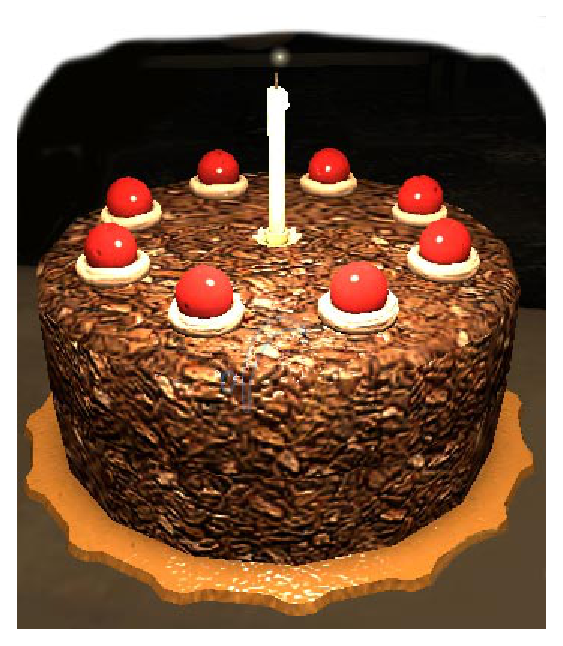
\includegraphics{party-cake.eps}
  \end{center}
\end{frame}

\begin{frame}
  \frametitle{Над задачей работали}
  \begin{itemize}
    \item Идея задачи: Глеб Евстропов
    \item Текст условия: Олег Давыдов
    \item Тесты, проверяющая программа и др.: Сергей Мельников
    \item Решения: Сергей Мельников, Антон Банных, Олег Давыдов
    \item Текст разбора: Олег Давыдов
  \end{itemize}
\end{frame}

\begin{frame}
  \frametitle{Формулировка задачи}
  \begin{itemize}
    \item Дано $n$ друзей, из них надо выбрать некоторое подмножество
    \item У каждого из друзей есть ограничения в обе стороны на размер доли, то есть, на количество выбранных друзей
      \begin{itemize}
        \item Если $i$-й друг может заплатить от $a_i$ до $b_i$, то он может быть в группе приглашённых размером
              от~$\lceil\frac{S}{b_i}\rceil-1$~до~$\lfloor\frac{S}{a_i}\rfloor-1$ человек
      \end{itemize}
    \item Нужно максимизировать суммарное веселье
  \end{itemize}
\end{frame}

\begin{frame}
  \frametitle{Идея решения}
  \begin{itemize}
    \item Если известно число $k$ (количество пришлашённых друзей), то задача решается очень просто: из всех друзей,
          которых мы можем взять в группу размера $k$, надо выбрать $k$ друзей с максимальным весельем
    \item Можно перебрать все различные $k$
    \item Но ограничения не позволяют перебрать всех друзей для каждого $k$, так что надо научиться быстро узнавать
          сумму $k$ максимальных по веселью допустимых друзей
  \end{itemize}
\end{frame}

\begin{frame}
  \frametitle{Как это сделать}
  \begin{itemize}
    \item Отсортируем всех друзей в порядке уменьшения веселья: теперь всегда надо брать просто $k$ первых допустимых друзей
    \item Будем перебирать $k$ в порядке увеличения и следить за множеством допустимых друзей
      \begin{itemize}
        \item Тогда каждый друг будет один раз добавлен в наше множество и один раз удалён из него
        \item Чтобы это сделать, достаточно выписать для каждого друга два события: его появление и его уход; упорядочим эти
              события по их <<времени>>, то есть по граничному размеру группы
        \item Такой подход (выписать события и их отсортировать) часто встречается в задачах по программированию
      \end{itemize}
    \item Осталось научиться брать сумму $k$ первых друзей из допустимого множества. 
    Для этого можно применить какую-нибудь структуру данных
  \end{itemize}
\end{frame}

\begin{frame}
  \frametitle{Структура данных}
  \begin{itemize}
    \item Такая структура данных "--- любое сбалансированное дерево 
    (например, декартово). Ключом в дереве будет номер друга
    \item Каждая вершина дерева должна хранить сумму веселья и количество 
    вершин в поддереве. Эти значения нужно будет
          пересчитывать в операциях, изменяющих дерево
    \item Помимо обычных операций (добавление и удаление элемента) понадобится 
    ещё одна "--- подсчитать сумму веселья на первых $k$ вершинах.
          Именно для этого мы стали хранить сумму на поддереве и его размер.
  \end{itemize}
\end{frame}

\begin{frame}
  \frametitle{Альтернативный вариант}
  \begin{itemize}
    \item Такая структура данных "--- два дерева отрезков
    \item Оба дерева отрезков будут считать суммы на массиве из $n$ элементов
    \item В первом дереве отрезков будем хранить $1$ или $0$ для каждого друга, 
    в зависимости от того, есть ли друг в множестве
    \item Во втором дереве для друга из множеста будем хранить его веселье $f_i$, 
    а для друга не из множества "--- ноль.
    \item Сумма веселья первых $k$ допустимых друзей считается в два этапа:
      \begin{itemize}
        \item С помощью первого дерева подсчитаем номер $k$-го друга из множества
        \item Зная нужный индекс, возьмём сумму на отрезке во втором дереве
      \end{itemize}
  \end{itemize}
\end{frame}

\begin{frame}
  \frametitle{Итого}
  \begin{itemize}
    \item Мы получили решение, работающее за $O(n\log{n})$ и использующее $O(n)$ памяти
    % \item % Сюда можно вставить статистику, если будет время после контеста
    \item Различные решения жюри занимают от трёх до шести килобайт, 
    что довольно много для олимпиадной задачи
    \item Домашнее задание: придумать решение за $O(n\sqrt{n})$
    \item Вопросы?
  \end{itemize}
\end{frame}

